\chapter{Forskningsmetoder}
\label{ch:method}
Dette kapittelet redegjør for forskningsmetodene til prosjektet. Forskningsstrategiene og datagenereringsmetodene
tar utgangspunkt i \citet{oates}.

\section{Forskningsstrategier}

\subsection{Design og kreasjon}
\textquote[\cite{oates}]{Forskningsmetoden design og kreasjon fokuserer på utvikling av nye IT-produkter, også kalt \textit{artefakter}.
Typer IT-artifakter inkluderer (March \& Smith, 1995): begreper, modeller, metoder og implementasjoner}{.}
Hovedpoenget er å lære gjennom å lage, og \citet{oates} identifiserer fem steg for denne prosessen:

\begin{description}
  \item[Bevisstgjøring] Hva er problemet?
  \item[Forslag] Hvordan kan problemet løses?
  \item[Utvikling] Problemløsingsfasen
  \item[Evaluering] Hvordan gikk dette?
  \item[Konklusjon] Hva kan vi trekke ut av dette?
\end{description}

\subsection{Case-studie}
\textquote[\cite{oates}]{En eksempelstudie fokuserer på én instans av det som skal undersøkes: en organisasjon, en avdeling, et informasjonssystem,
    et diskusjonsforum (...). Denne ene instansen, eller tilfellet, studeres i detalj med forskjellige datagenereringsmetoder som
    intervju, observasjon, dokumenter (...)}{.}
    
\subsection{Prototyping}

\subsection{Brukersentrert utvikling}
Brukersentrert utvikling er en prosess der brukeren er involvert i hvert steg.
Stegene er å forstå brukskonteksten, etablere krav, implementere artefakt og evaluere artefakt. Dette er en syklus som kan gjentas flere ganger.
\citet{dis20099241} standardiserer brukersentrert utvikling. Se figur \ref{fig:iso9241-210}
for de ulike stegene i prosessen.
Brukersentrert utvikling passer godt i de fem stegene som inngår i «design og kreasjon»-forskningsmetoden.

\begin{figure}
\centering
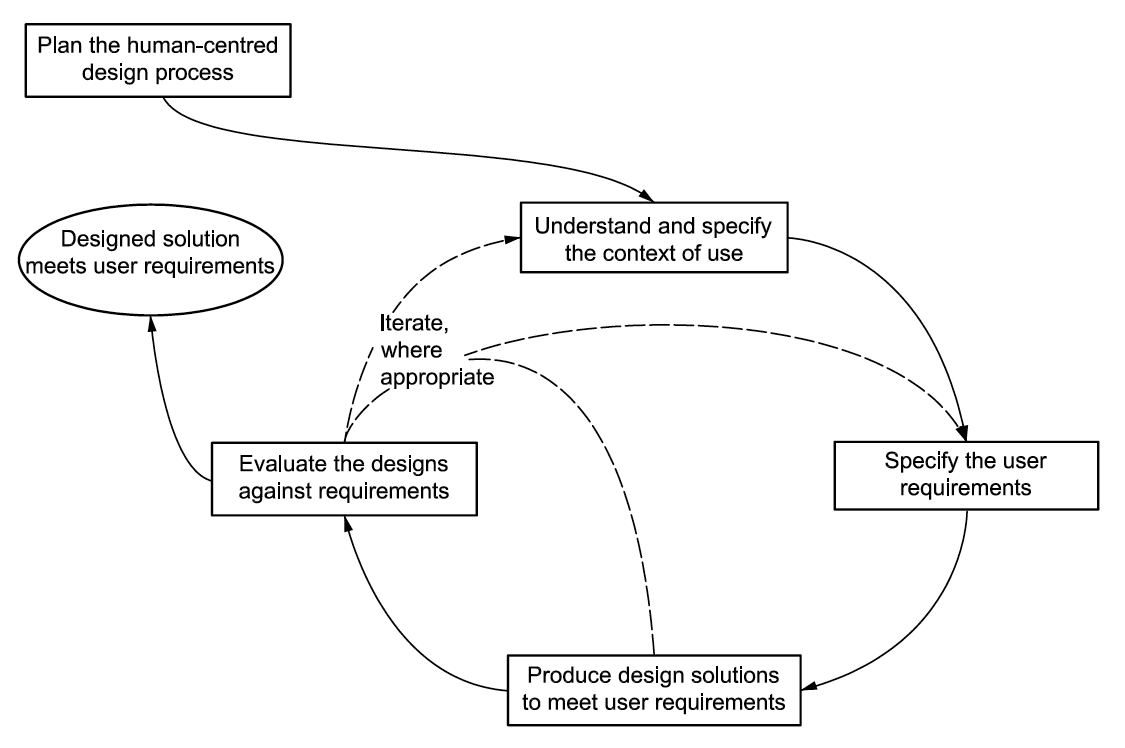
\includegraphics[width=0.85\textwidth]{fig/iso9241-210}
\caption{Gjensidige avhengigheter innenfor menneskeorientert designaktiviteter \citep{dis20099241}.}
\label{fig:iso9241-210}
\end{figure}

\section{Datagenereringsmetoder}

\subsection{Semistrukturert intervju}

\subsection{Dokumenter}